% Provenance (never printed): see sources/outline_sources.md (Year 2: mid-latitude cyclones and
% fronts; jets and Rossby waves, descriptive; tropical cyclones; numerical weather prediction,
% principle). Definitions after the NWS glossary and UCAR; cyclogenesis conditions after the NOAA
% AOML FAQ; potential intensity after Gilford (2021, pyPI); conveyor belts after Raveh-Rubin and
% Catto (2019); blocking after Wang and others (2026); predictability after Krishnamurthy (2019),
% Selz and others (2022) and ECMWF. The Lorenz system from figdata/bachelor-2/weather.py; the
% fronts, waves and storms of the examples, exercises and problem are invented, their values
% computed in the Book 4 scratch calculator calc/ch22.py.
\chapter{Sistem Cuaca}\label{ch:b2:weather-systems}

Prakiraan untuk empat hari ke depan kini sama tepatnya dengan prakiraan untuk satu hari ke depan tiga puluh
tahun yang lalu, dan setiap dasawarsa telah menambahkan sekitar satu hari prakiraan yang berguna. Namun tidak ada prakiraan
cuaca pada hari tertentu, di tempat tertentu, yang dapat diandalkan jauh melampaui sepuluh hari, dan komputer yang lebih baik
saja tidak akan mendorong batas itu jauh: atmosfer memperbesar ketidakpastiannya sendiri yang kecil. Bab
ini menggambarkan sistem-sistem cuaca yang diikuti oleh prakiraan, yaitu front dan depresi di
lintang tengah, gelombang arus jet, dan siklon tropis, lalu cara sistem-sistem itu
diprakirakan dan mengapa prakiraan harus berhenti di suatu titik.
% ledger: mo:accuracy, bauer:day-per-decade, krish19:predictability

\begin{recall}
\textbf{Dari volume-volume sekolah}: massa udara, front, front dingin dan front hangat, depresi dan
antisiklon, isobar dan prakiraan cuaca; siklon tropis, matanya dan dinding matanya,
skala Saffir--Simpson. \textbf{Dari volume Tahun 1}: gaya gradien tekanan,
parameter Coriolis $f = 2\Omega\sin\varphi$, keseimbangan geostrofik, siklon dan antisiklon,
ketiga sel, angin baratan, dan arus jet. \textbf{Dari buku-buku fisika}: mesin kalor
dan efisiensi siklus Carnot. \textbf{Dari \cref{ch:b2:atmospheric-thermodynamics}}:
kejenuhan, \omterm{def:b2:atmospheric-thermodynamics:moist-adiabat}{adiabat lembap}, $\theta_e$, \omterm{def:b2:atmospheric-thermodynamics:instability}{ketidakstabilan bersyarat}, dan CAPE.
\end{recall}

\section{Front}\label{sec:b2:weather-systems:fronts}

Volume-volume sekolah menggambar front sebagai garis pada peta. Front adalah garis tempat batas miring
antara dua massa udara bertemu dengan permukaan tanah, dan cuacanya berasal dari kemiringan itu.

\begin{definition}[Bidang front; front stasioner; front oklusi]\label{def:b2:weather-systems:fronts}
Yang disebut \emph{bidang front}\index{bidang front} suatu front adalah batas miring antara
kedua massa udara, dengan massa yang lebih padat dan lebih dingin terletak di bawah sebagai baji; front pada peta adalah
perpotongannya dengan permukaan tanah. Yang disebut \emph{front stasioner}\index{front stasioner} adalah front
yang bergerak sangat lambat atau tidak bergerak sama sekali. Yang disebut \emph{front oklusi}\index{front oklusi} adalah
gabungan dua front, yang terbentuk ketika front dingin menyusul front hangat atau front stasioner.
\end{definition}
% ledger: nws4:front, nws4:stationary, nws4:occluded

\omterm{def:b2:weather-systems:fronts}{Front stasioner} terbentuk ketika tidak satu pun massa udara dapat mendorong yang lain, dan angin bertiup di sepanjang
front, bukan melintasinya; front itu dapat bertahan berhari-hari, berawan dan basah, sebelum bergerak lagi sebagai front dingin
atau front hangat. Pada peta, front itu berselang-seling antara segitiga biru front dingin, yang menunjuk ke arah
udara hangat, dan setengah lingkaran merah front hangat, yang menunjuk ke arah udara dingin. \omterm{def:b2:weather-systems:fronts}{Front
oklusi} digambar dengan warna ungu dengan kedua simbol pada sisi yang sama. Bila udara di belakang front dingin
lebih dingin, udara itu menyusup di bawah front hangat dan mengangkatnya ke atas, yaitu oklusi dingin; bila udara
di depan front hangat lebih dingin, front dingin naik di atasnya, yaitu oklusi hangat.
% ledger: ucar4:stationary-occluded, nws4:occluded

Seberapa curam \omterm{def:b2:weather-systems:fronts}{bidang front}? Jawabannya menggabungkan kesetimbangan hidrostatik dengan keseimbangan
geostrofik pada volume Tahun 1.

\begin{proposition}[Kemiringan bidang front]\label{prop:b2:weather-systems:slope}
Misalkan sebuah \omterm{def:b2:weather-systems:fronts}{bidang front} memisahkan udara dingin bersuhu $T_c$ dari udara hangat bersuhu $T_w$, dengan
angin geostrofik $v_c$ dan $v_w$ di sepanjang front. Ambil sumbu $x$ melintasi front ke arah
udara dingin dan sumbu $y$ di sepanjangnya, sehingga $(x, y, z)$ bersistem tangan kanan. Maka \omterm{def:b2:weather-systems:fronts}{bidang
front} naik ke arah udara dingin dengan kemiringan
\[
  \tan\alpha \approx \frac{f\,\bar T\,(v_c - v_w)}{g\,(T_w - T_c)},
\]
dengan $\bar T$ suhu rata-rata. \omterm{def:b2:weather-systems:fronts}{Bidang front} yang setimbang memerlukan lompatan angin
di sepanjangnya, $v_c > v_w$: angin berbelok secara siklonik melintasi front.
\end{proposition}

\begin{proof}
Tekanan bersifat kontinu melintasi \omterm{def:b2:weather-systems:fronts}{bidang front}, sehingga perubahannya di sepanjang bidang itu
sama bila dihitung pada kedua sisinya: $\partial_x p_c\,\mathrm{d}x + \partial_z p_c\,\mathrm{d}z =
\partial_x p_w\,\mathrm{d}x + \partial_z p_w\,\mathrm{d}z$. Pada setiap sisi $\partial_z p = -\rho g$
(kesetimbangan hidrostatik) dan $\partial_x p = \rho f v$ (keseimbangan geostrofik). Jadi
$\rho_c f v_c\,\mathrm{d}x - \rho_c g\,\mathrm{d}z = \rho_w f v_w\,\mathrm{d}x - \rho_w
g\,\mathrm{d}z$, dan
\[
  \frac{\mathrm{d}z}{\mathrm{d}x} = \frac{f(\rho_c v_c - \rho_w v_w)}{g(\rho_c - \rho_w)} .
\]
Pada tekanan yang sama, $\rho \propto 1/T$, sehingga $\rho_c - \rho_w \approx \bar\rho\,(T_w -
T_c)/\bar T$; dalam pembilang, selisih densitas yang kecil dapat diabaikan, yang
memberikan rumusnya. Udara dingin terletak di bawah, sehingga bidang itu naik ke arahnya, $\mathrm{d}z/
\mathrm{d}x > 0$, dan $v_c > v_w$. Dengan $x$ ke arah udara dingin, vortisitas relatif
$\partial v/\partial x$ melintasi front lalu bernilai positif: siklonik.
\end{proof}

\begin{example}[Kemiringan yang khas]\label{ex:b2:weather-systems:slope}
Pada \ang{45} LU, $f = \qty{1.03e-4}{s^{-1}}$. Melintasi front dengan $\bar T = \qty{280}{K}$,
kontras suhu \qty{5}{K}, dan angin yang berubah \qty{10}{m/s} di sepanjangnya, $\tan\alpha
= 1.03 \times 10^{-4} \times 280 \times 10/(9.81 \times 5) = 0.0059$, sekitar 1 banding 170: \omterm{def:b2:weather-systems:fronts}{bidang
front} mencapai ketinggian \qty{1}{km} sekitar \qty{170}{km} dari front di permukaan tanah.
Perubahan angin yang lebih tajam memberikan bidang yang lebih curam; kontras suhu yang lebih kuat, bidang yang lebih landai.
\end{example}

Front yang sebenarnya memiliki kemiringan dengan orde ini, dan baji yang landai itu menjelaskan cuacanya. Di depan
front hangat, udara hangat meluncur naik pada lereng landai sepanjang ratusan kilometer: awan tinggi,
sirus dan sirostratus, datang lebih dahulu, lalu altostratus, dan awan menebal dan merendah sampai
hujan turun dekat front. Front dingin, yang lebih curam dan lebih cepat, sampai dua kali lebih cepat daripada front
hangat, mengangkat udara hangat secara mendadak: kumulus dan kumulonimbus, hujan deras sesaat, embusan angin, dan penurunan
suhu yang tiba-tiba, dengan tekanan yang berhenti turun dan mulai naik ketika front lewat. Front
tempat udara hangat menuruni \omterm{def:b2:weather-systems:fronts}{bidang front} alih-alih menaikinya disebut katafront.
% ledger: ucar:warm-front, ucar:cold-front, nws4:front

\begin{omfigure}
\centering
\begin{tikzpicture}[font=\scriptsize, >=Stealth, x=1cm, y=1cm]
% air masses
\fill[omCold!12] (0,0) -- (0,3.4) .. controls (1.6,2.2) and (3.2,0.8) .. (4,0) -- cycle;
\fill[omCold!12] (9.6,0) .. controls (11,0.6) and (12.6,1.5) .. (14,2.4) -- (14,0) -- cycle;
\fill[omWarm!8] (4,0) .. controls (3.2,0.8) and (1.6,2.2) .. (0,3.4) -- (0,4.8) -- (14,4.8)
  -- (14,2.4) .. controls (12.6,1.5) and (11,0.6) .. (9.6,0) -- cycle;
% frontal surfaces
\draw[omCold, thick] (4,0) .. controls (3.2,0.8) and (1.6,2.2) .. (0,3.4);
\draw[omWarm, thick] (9.6,0) .. controls (11,0.6) and (12.6,1.5) .. (14,2.4);
% clouds
\fill[black!18, draw=black!45] (3.75,0.5) .. controls (3.5,1.8) and (3.7,3.2) .. (3.9,3.9)
  .. controls (3.2,4.15) and (3.0,4.5) .. (3.4,4.6) -- (5.8,4.6) .. controls (6.1,4.45) and
  (5.7,4.15) .. (5.1,3.9) .. controls (5.3,3.0) and (5.4,1.6) .. (5.05,0.5) -- cycle;
\node[align=center] at (4.45,2.6) {kumulo-\\nimbus};
\fill[black!15, draw=black!40] (9.6,0.35) .. controls (10.4,0.75) and (11.2,1.05) .. (11.9,1.25)
  -- (11.9,1.75) .. controls (11,1.6) and (10.2,1.35) .. (9.4,0.95) -- cycle;
\node at (10.75,1.25) [rotate=21] {nimbostratus};
\fill[black!10, draw=black!35] (11.9,1.35) .. controls (12.3,1.55) and (12.7,1.75) .. (13.0,1.9)
  -- (13.0,2.25) .. controls (12.6,2.1) and (12.2,1.95) .. (11.9,1.85) -- cycle;
\node[anchor=south] at (12.45,2.15) {altostratus};
\draw[black!40, line width=1.6pt] (12.9,2.75) -- (13.9,3.05);
\node[anchor=south] at (13.35,3.05) {sirostratus};
\foreach \x in {12.2,12.7,13.2,13.7} {\draw[black!40, thick] (\x,3.95) .. controls (\x+0.15,4.05) .. (\x+0.35,3.9);}
\node[anchor=south] at (13.0,4.05) {sirus};
% rain
\foreach \x in {3.95,4.25,4.55,4.85} {\draw[omCold!70, dashed] (\x,0.45) -- (\x-0.12,0.02);}
\foreach \x in {9.8,10.2,10.6,11.0,11.4} {\draw[omCold!70, dashed] (\x,0.55) -- (\x-0.12,0.02);}
% ground and labels
\draw[thick] (0,0) -- (14,0);
\node at (1.2,0.8) {udara dingin};
\node at (7.0,2.4) {sektor hangat};
\node at (12.8,0.55) {udara dingin};
\node[anchor=north, omCold] at (4,-0.05) {front dingin};
\node[anchor=north, omWarm] at (9.6,-0.05) {front hangat};
\draw[->, thick] (6.0,0.55) -- (7.2,0.55) node[right] {front bergerak ke timur};
\draw[->, black!60] (5.8,1.1) .. controls (7.0,1.4) and (9.5,2.0) .. (12.2,3.3);
\node[black!60, rotate=13] at (8.4,2.0) {udara hangat meluncur naik};
\end{tikzpicture}
\par\smallskip{\small Penampang melalui front dingin dan front hangat, dengan barat di sebelah kiri
(skematis: skala vertikal dilebih-lebihkan sekitar seratus kali, dan front dingin digambar
lebih curam daripada front hangat). Nama dan urutan awan seperti dalam teks.}
\end{omfigure}
% ledger: ucar:warm-front, ucar:cold-front

\section{Siklon ekstratropis}\label{sec:b2:weather-systems:cyclones}

\begin{definition}[Siklon ekstratropis; model front kutub; siklogenesis]\label{def:b2:weather-systems:cyclones}
Yang disebut \emph{siklon ekstratropis}\index{siklon ekstratropis} adalah siklon di lintang tengah dan lintang
tinggi, yang sering berdiameter sekitar \qty{2000}{km}, dan biasanya mengandung front, dengan front dingin yang menjulur
sepanjang ratusan kilometer ke arah khatulistiwa. \emph{Model front kutub}\index{model front kutub}
menggambarkan kehidupannya sebagai gelombang yang tumbuh pada front kutub, yaitu front panjang antara udara kutub
dan udara tropis. Yang disebut \emph{siklogenesis}\index{siklogenesis} adalah pembentukan atau penguatan
suatu siklon.
\end{definition}
% ledger: nws4:extratropical, nws4:polar-front

Model itu mengikuti siklon melalui empat tahap, seperti yang digambar pada gambar di bawah. \omterm{def:b2:weather-systems:fronts}{Front
stasioner} memisahkan udara dingin yang bergerak ke barat di sisi kutubnya dari udara hangat yang bergerak ke timur di sisi
khatulistiwanya. Suatu gangguan membengkokkan front menjadi gelombang; tekanan turun di puncaknya,
daerah tekanan rendah terbentuk, dan front di sebelah timur daerah itu maju ke arah kutub sebagai front hangat, sedangkan front di sebelah barat
daerah itu maju ke arah khatulistiwa sebagai front dingin. Di antara keduanya terletak sektor hangat. Front dingin
bergerak lebih cepat daripada front hangat, sektor hangat menyempit, dan front dingin menyusul front
hangat dekat pusat tekanan rendah: oklusi menyebar ke luar dari pusat, mengangkat udara hangat dari
permukaan tanah, dan siklon itu, yang terputus dari pasokan udara hangatnya, terisi dan mati. Titik tempat
ketiga front bertemu disebut titik tripel. Pada citra satelit, siklon yang matang menunjukkan
awan berbentuk koma, dan celah kering berupa udara cerah yang melingkar masuk ke sisi selatan dan timurnya.
% ledger: nws4:extratropical, nws4:occluded, ucar:cold-front

\begin{omfigure}
\centering
\begin{tikzpicture}[font=\scriptsize, >=Stealth]
% (a) stationary front
\begin{scope}[shift={(0,4.1)}]
\draw[black!30] (0,0) rectangle (6.4,3.4);
\node[anchor=north west] at (0,3.4) {\textbf{a}\enspace front stasioner};
\draw[stationary front] (6.1,1.6) -- (0.3,1.6);
\draw[->, black!60] (4.2,2.5) -- (2.2,2.5); \node[black!60] at (3.2,2.8) {udara dingin};
\draw[->, black!60] (2.2,0.7) -- (4.2,0.7); \node[black!60] at (3.2,0.4) {udara hangat};
\end{scope}
% (b) open wave
\begin{scope}[shift={(6.9,4.1)}]
\draw[black!30] (0,0) rectangle (6.4,3.4);
\node[anchor=north west] at (0,3.4) {\textbf{b}\enspace gelombang dan tekanan rendah};
\fill[omWarm!10] (3.0,1.9) .. controls (3.9,1.75) and (4.8,1.55) .. (6.0,1.4) -- (6.0,0.2)
  -- (1.3,0.2) .. controls (2.0,0.9) and (2.6,1.4) .. (3.0,1.9) -- cycle;
\draw[black!45] (3.0,1.9) ellipse (0.55 and 0.4);
\draw[black!45] (3.0,1.9) ellipse (1.05 and 0.75);
\draw[warm front] (3.0,1.9) .. controls (3.9,1.75) and (4.8,1.55) .. (6.0,1.4);
\draw[cold front] (3.0,1.9) .. controls (2.6,1.4) and (2.0,0.9) .. (1.3,0.2);
\node[font=\small\bfseries, omWarm!70!black] at (2.7,2.15) {L};
\node at (4.5,0.75) {sektor hangat};
\end{scope}
% (c) mature
\begin{scope}[shift={(0,0)}]
\draw[black!30] (0,0) rectangle (6.4,3.4);
\node[anchor=north west] at (0,3.4) {\textbf{c}\enspace siklon matang};
\fill[omWarm!10] (3.0,1.9) .. controls (3.9,1.7) and (4.8,1.5) .. (6.0,1.25) -- (6.0,0.2)
  -- (3.3,0.2) .. controls (3.3,0.8) and (3.2,1.45) .. (3.0,1.9) -- cycle;
\draw[black!45] (3.0,1.9) ellipse (0.5 and 0.36);
\draw[black!45] (3.0,1.9) ellipse (0.95 and 0.66);
\draw[black!45] (3.0,1.9) ellipse (1.4 and 0.95);
\draw[warm front] (3.0,1.9) .. controls (3.9,1.7) and (4.8,1.5) .. (6.0,1.25);
\draw[cold front] (3.0,1.9) .. controls (3.2,1.45) and (3.3,0.8) .. (3.3,0.2);
\node[font=\small\bfseries, omWarm!70!black] at (2.7,2.15) {L};
\node at (4.9,0.65) {sektor hangat};
\end{scope}
% (d) occluded
\begin{scope}[shift={(6.9,0)}]
\draw[black!30] (0,0) rectangle (6.4,3.4);
\node[anchor=north west] at (0,3.4) {\textbf{d}\enspace oklusi};
\fill[omWarm!10] (4.0,1.55) .. controls (4.6,1.45) and (5.3,1.3) .. (6.1,1.1) -- (6.1,0.2)
  -- (4.6,0.2) .. controls (4.5,0.7) and (4.3,1.2) .. (4.0,1.55) -- cycle;
\draw[black!45] (2.5,1.95) ellipse (0.5 and 0.36);
\draw[black!45] (2.5,1.95) ellipse (0.95 and 0.66);
\draw[black!45] (2.5,1.95) ellipse (1.45 and 0.95);
\draw[occluded front] (2.5,1.95) .. controls (3.0,1.9) and (3.6,1.75) .. (4.0,1.55);
\draw[warm front] (4.0,1.55) .. controls (4.6,1.45) and (5.3,1.3) .. (6.1,1.1);
\draw[cold front] (4.0,1.55) .. controls (4.3,1.2) and (4.5,0.7) .. (4.6,0.2);
\node[font=\small\bfseries, omWarm!70!black] at (2.2,2.2) {L};
\node[anchor=north east, align=right, fill=white, inner sep=1pt] at (3.9,1.3) {titik\\tripel};
\fill (4.0,1.55) circle (0.6mm);
\end{scope}
\end{tikzpicture}
\par\smallskip{\small Kehidupan \omterm{def:b2:weather-systems:cyclones}{siklon ekstratropis} dalam \omterm{def:b2:weather-systems:cyclones}{model front kutub}, Belahan Bumi
Utara, utara di atas (skematis): \omterm{def:b2:weather-systems:fronts}{front stasioner} (a); gelombang dengan tekanan rendah di puncaknya,
front hangat dan front dingin dengan sektor hangat di antaranya (b); front dingin menyusul
(c); \omterm{def:b2:weather-systems:fronts}{front oklusi} tumbuh dari pusat (d). Elips hitam: isobar.}
\end{omfigure}
% ledger: nws4:occluded, nws4:extratropical, ucar4:stationary-occluded

Front-front dalam model itu hanyalah jejak permukaan dari aliran-aliran udara siklon, yang
digambarkan para ahli meteorologi sebagai tiga arus: sabuk konveyor hangat, yaitu udara lembap yang naik dari
sektor hangat di depan front dingin; sabuk konveyor dingin di sisi dingin front; dan
intrusi kering, yaitu arus udara dari troposfer atas, kadang-kadang dari stratosfer paling bawah,
yang turun ke arah permukaan di belakang front dingin dan menyebar dekat
permukaan tanah.
% ledger: rr19:conveyor

Dari mana energi suatu siklon berasal? Bukan dari kalor laten saja, seperti pada badai guntur,
tetapi dari kontras suhu antara udara kutub dan udara tropis. Siklon lintang tengah
menguat di zona baroklinik, tempat suhu berubah secara horizontal pada permukaan bertekanan
tetap dan angin berubah terhadap ketinggian. Siklon yang tumbuh membawa udara hangat ke arah kutub
dan ke atas serta udara dingin ke arah khatulistiwa dan ke bawah: siklon itu menurunkan pusat massa
atmosfer dan mengubah energi potensial menjadi energi kinetik angin-anginnya. Volume Tahun~3
mengkaji perubahan itu.
% ledger: nws4:extratropical

\begin{omfigure}
\centering
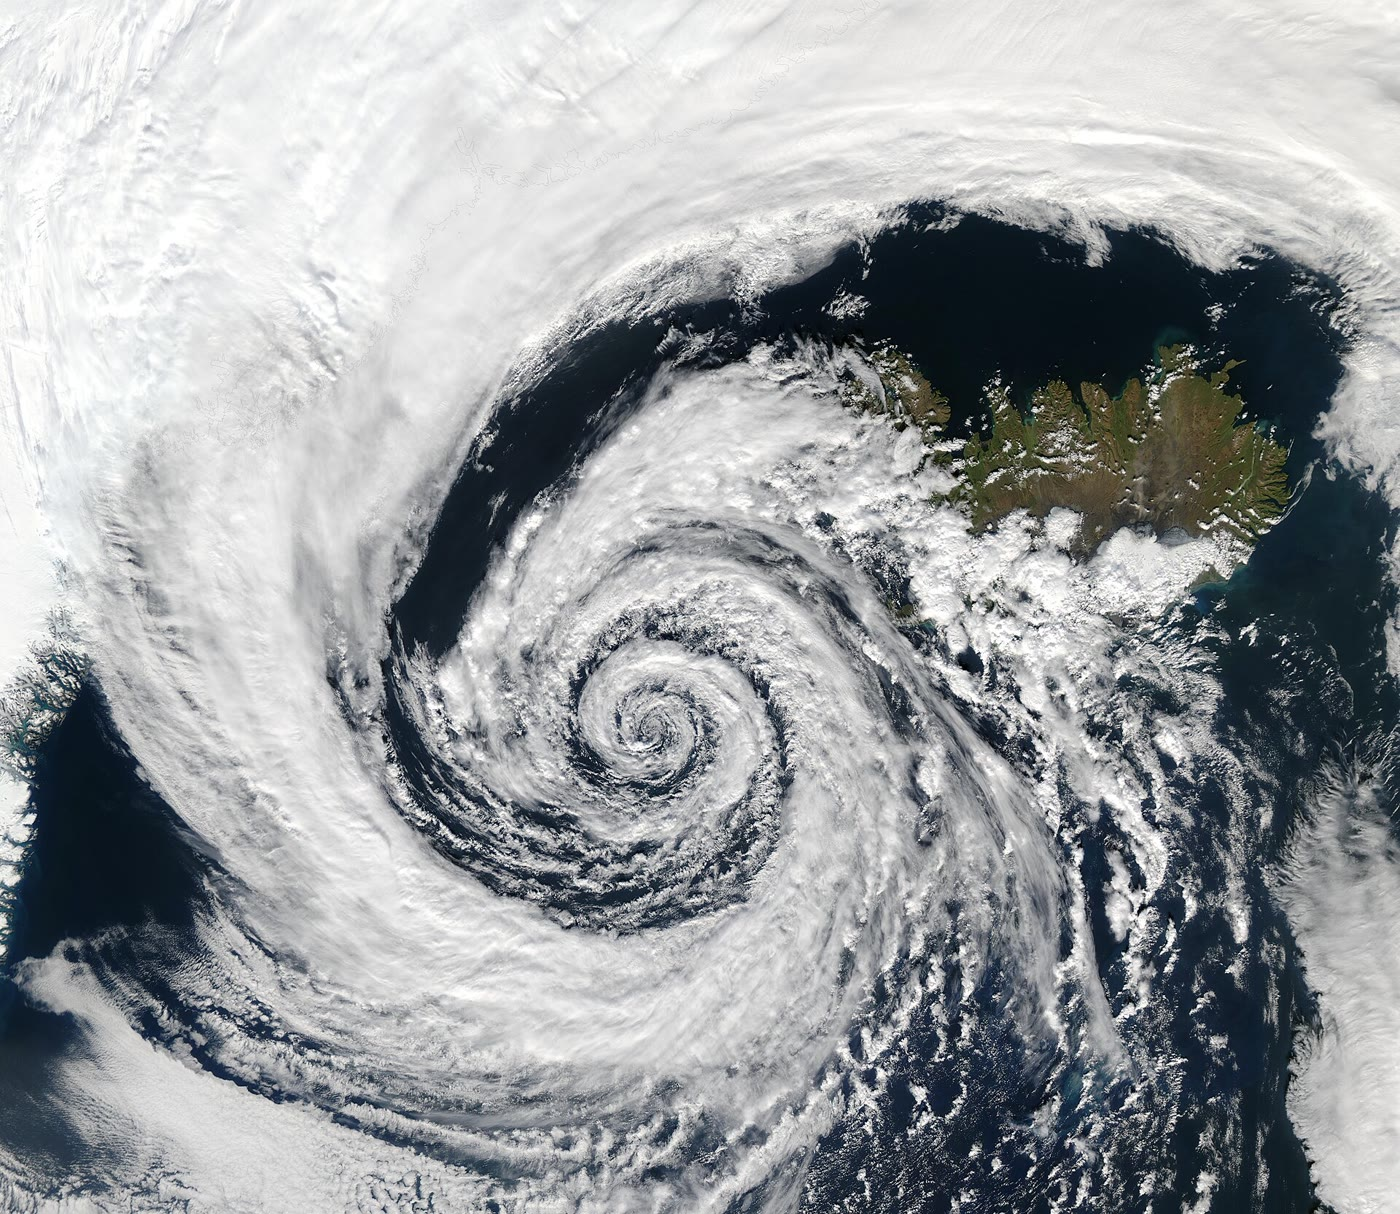
\includegraphics[width=0.58\linewidth]{images/book4/b2-22-iceland-low.jpg}
\par\smallskip{\small Daerah tekanan rendah yang dalam di lepas pantai barat daya Islandia, 4 September 2003, dilihat oleh
instrumen MODIS pada satelit Aqua milik NASA: pita-pita awan berpilin masuk ke pusat. (Foto: NASA
Goddard Space Flight Center, MODIS Rapid Response Team dan Jacques Descloitres, domain publik, via
Wikimedia Commons.)}
\end{omfigure}

\section{Arus jet dan gelombang Rossby}\label{sec:b2:weather-systems:rossby}

Siklon tidak tersebar secara acak. Arus jet kutub, yaitu inti cepat angin baratan di atas front
kutub, berkaitan dengan kedudukan dan gerak daerah tekanan tinggi dan tekanan rendah di lintang
tengah; arus itu paling cepat di sepanjang jet streak-nya, yaitu bentangan tempat kecepatan anginnya memuncak, dan arus itu
tidak mengitari kutub sebagai cincin: arus itu berkelok-kelok.
% ledger: nws4:polar-front, nws4:jet-streak

\begin{definition}[Gelombang Rossby; palung dan punggungan udara atas]\label{def:b2:weather-systems:rossby}
Yang disebut \emph{gelombang Rossby}\index{gelombang Rossby} adalah gelombang aliran angin baratan di troposfer atas,
yaitu deretan palung dan punggungan sepanjang ribuan kilometer dengan amplitudo utara--selatan yang besar.
Yang disebut \emph{palung udara atas}\index{palung udara atas} adalah daerah memanjang yang tekanannya relatif rendah
dalam gelombang seperti itu, tempat aliran membelok ke arah khatulistiwa; \emph{punggungan udara atas}\index{punggungan udara atas}
adalah daerah memanjang yang tekanannya relatif tinggi, tempat aliran itu
membelok ke arah kutub.
\end{definition}
% ledger: nws4:rossby

\omterm{def:b2:weather-systems:rossby}{Gelombang Rossby} ada karena parameter Coriolis bertambah ke arah kutub. Udara yang terdorong ke arah kutub
mendapati $f$ yang lebih besar dan, dengan mempertahankan vortisitas mutlaknya, berbalik ke arah khatulistiwa; udara yang
terdorong ke arah khatulistiwa berbalik ke arah kutub. Laju pertambahan $f$ ke utara,
$\beta = \mathrm{d}f/\mathrm{d}y = 2\Omega\cos\varphi/a$ dengan $a$ jari-jari Bumi, menentukan
kecepatannya. Volume Tahun~3 menurunkan, dari kekekalan vortisitas, kecepatan fase
gelombang dengan panjang gelombang $\lambda$ dalam angin baratan seragam $U$:
\[
  c = U - \frac{\beta}{k^2}, \qquad k = \frac{2\pi}{\lambda} .
\]
Terimalah rumus ini di sini. Terhadap udara, setiap \omterm{def:b2:weather-systems:rossby}{gelombang Rossby} bergerak ke barat, dan makin panjang gelombangnya, makin
cepat geraknya; angin membawanya ke timur. Gelombang pendek terbawa ke timur hampir secepat angin,
sedangkan gelombang panjang hanyut perlahan, diam di tempat, atau bahkan bergerak ke barat.
% ledger: earth:Trot, earth:Rmean

\begin{example}[Tiga gelombang pada 45° LU]\label{ex:b2:weather-systems:rossby}
Dengan $\Omega = \qty{7.292e-5}{s^{-1}}$ (satu hari sideris \qty{23.9345}{h}) dan $a =
\qty{6371}{km}$, $\beta = \qty{1.62e-11}{m^{-1}.s^{-1}}$ pada \ang{45} LU. Dalam angin baratan
\qty{15}{m/s}, gelombang \qty{4000}{km} memiliki $\beta/k^2 = \qty{6.6}{m/s}$ dan bergerak ke timur dengan kecepatan
\qty{8.4}{m/s}; gelombang \qty{6000}{km} memiliki $\beta/k^2 = \qty{14.8}{m/s}$ dan nyaris tidak bergerak, dengan
\qty{0.2}{m/s}; gelombang \qty{8000}{km} bergerak ke barat dengan kecepatan \qty{11.2}{m/s}.
\end{example}
% ledger: earth:Trot, earth:Rmean

Palung gelombang panjang bergerak lambat dan bertahan lama; gelombang pendek yang melintas melalui
palung itu, yaitu palung gelombang pendek, memicu udara naik di depannya, di sisi timurnya, tempat
tekanan permukaan turun dan daerah tekanan rendah berkembang. Palung yang sumbunya miring dari tenggara ke barat laut
sering menjadi tanda sistem yang sedang berkembang atau menguat.
% ledger: nws4:rossby

\begin{omfigure}
\centering
\begin{tikzpicture}[font=\scriptsize, >=Stealth]
\foreach \lat/\pa in {30/-72, 45/-72, 60/-108} {
  \pgfmathsetmacro{\r}{6.0*tan((90-\lat)/2)}
  \draw[black!25] (0,0) circle (\r);
  \node[black!50, fill=white, inner sep=1pt] at (\pa:\r) {\ang{\lat} LU};
}
\fill (0,0) circle (0.6mm);
\node[anchor=north, black!60] at (0,-0.08) {Kutub Utara};
\draw[ocBlue, very thick, smooth, samples=241, domain=0:360]
  plot ({6.0*tan((90-(47+11*cos(5*\x)))/2)*cos(\x)}, {6.0*tan((90-(47+11*cos(5*\x)))/2)*sin(\x)});
\foreach \a in {18, 90, 162, 234, 306} {
  \pgfmathsetmacro{\ra}{6.0*tan((90-(47+11*cos(5*\a)))/2)}
  \pgfmathsetmacro{\rb}{6.0*tan((90-(47+11*cos(5*(\a+2))))/2)}
  \draw[ocBlue, very thick, -{Stealth[length=2.6mm]}] (\a:\ra) -- (\a+2:\rb);
}
\pgfmathsetmacro{\rt}{6.0*tan((90-36)/2)}
\node[anchor=216, ocRed!80!black, inner sep=2pt] at (36:\rt) {palung};
\node[anchor=0, ocRed!80!black, inner sep=2pt] at (180:\rt) {palung};
\pgfmathsetmacro{\rr}{6.0*tan((90-58)/2)}
\node[anchor=72, ocRed!80!black, inner sep=3pt] at (72:\rr) {punggungan};
\end{tikzpicture}
\par\smallskip{\small \omterm{def:b2:weather-systems:rossby}{Gelombang Rossby} dalam arus jet yang dilihat dari atas Kutub Utara (skematis):
lima gelombang mengelilingi belahan bumi, dengan palung yang menjangkau ke arah khatulistiwa dan punggungan ke arah
kutub. Arus jet mengalir ke timur, berlawanan arah jarum jam bila dilihat dari atas kutub (panah). Lingkaran lintang
digambar seperti pada peta stereografis kutub.}
\end{omfigure}
% ledger: nws4:rossby

Kadang-kadang pola itu berhenti bergerak sama sekali.

\begin{definition}[Pemblokiran atmosfer]\label{def:b2:weather-systems:blocking}
Yang disebut \emph{pemblokiran atmosfer}\index{pemblokiran atmosfer} adalah sistem tekanan tinggi yang besar, bertahan lama, dan hampir
stasioner, kadang-kadang berpasangan dengan daerah tekanan rendah, yang memutus aliran normal arus jet ke arah
timur. Metode pendeteksian blok hampir semuanya mensyaratkan blok itu bertahan sedikitnya lima
hari.
\end{definition}
% ledger: wang26:blocking

Blok membelokkan arus jet dan siklon-siklon di sekelilingnya dan menahan cuaca yang sama di atas wilayah
yang sama selama berhari-hari: blok mendatangkan gelombang panas, kekeringan, kebakaran hutan, gelombang dingin, dan banjir di
lintang tengah. Pada akhir Juni dan awal Juli 2021 sebuah blok yang kuat menyebabkan gelombang panas di
Pacific Northwest, Amerika Utara, yang menimbulkan lebih dari seribu kematian. Proses-proses
fisika di balik pemblokiran masih belum dipahami dengan baik, dan model numerik kesulitan
mereproduksi seberapa sering blok terjadi dan berapa lama blok bertahan.
% ledger: wang26:blocking, wang26:gaps

\section{Siklon tropis}\label{sec:b2:weather-systems:tropical}

Siklon tropis tidak memiliki front dan tidak memiliki kontras suhu sebagai sumber energi. Siklon itu menarik energinya
dari samudra yang hangat, melalui kalor laten air yang diuapkannya, seperti yang diukur dalam \cref{ch:b2:atmospheric-thermodynamics}.
Enam kondisi mendukung pembentukannya: air samudra sedikitnya \qty{26.5}{\celsius}
sampai kedalaman berorde \qty{50}{m}; atmosfer yang mendingin cukup cepat terhadap ketinggian sehingga
tidak stabil bagi konveksi lembap; troposfer tengah yang lembap, sekitar \qty{5}{km}; jarak
sedikitnya sekitar \qty{500}{km} dari khatulistiwa, agar gaya Coriolis dapat menahan daerah tekanan rendah dalam
keseimbangan; gangguan yang sudah ada dekat permukaan; dan geser angin vertikal yang lemah, di bawah sekitar
\qty{10}{m/s} antara permukaan dan troposfer atas. Kondisi-kondisi itu perlu tetapi tidak
cukup: banyak gangguan yang memenuhinya tidak pernah berkembang.
% ledger: aoml:tc-genesis

Setelah terbentuk, siklon tropis adalah sebuah mesin kalor. Udara berpilin ke dalam di atas laut pada suhu yang hampir
tetap, sambil memperoleh kalor dan kelembapan dari samudra; di dinding mata udara itu naik
secara adiabatik; dalam aliran keluar dekat tropopause udara itu kehilangan kalor melalui radiasi pada suhu yang rendah
dan hampir tetap; dan udara itu turun lagi jauh dari pusat, menyelesaikan suatu siklus yang
menyerupai siklus Carnot. Usaha siklus itu menggerakkan angin melawan gesekan permukaan
laut.
% ledger: gilford21:pi

\begin{omfigure}
\centering
\begin{tikzpicture}[font=\scriptsize, >=Stealth, x=1cm, y=1cm]
% sea and axis
\fill[ocBlue!12] (0,-0.35) rectangle (12.5,0);
\draw[thick, ocBlue!70!black] (0,0) -- (12.5,0);
\node[anchor=north west, ocBlue!70!black] at (8.6,-0.02) {laut hangat, $T_s$};
\draw[dashed, black!50] (0,-0.35) -- (0,4.9);
\node[anchor=south, black!60] at (0,4.9) {pusat};
% eyewall cloud and outflow cloud
\fill[black!14, draw=black!40] (0.9,0.25) .. controls (0.7,1.8) and (0.75,3.3) .. (0.95,4.2)
  .. controls (3.5,4.55) and (7.0,4.45) .. (9.5,4.2) .. controls (7.0,3.9) and (3.6,3.85)
  .. (2.1,3.7) .. controls (1.95,2.6) and (1.9,1.4) .. (2.0,0.25) -- cycle;
\node[black!60] at (0.45,2.0) [rotate=90] {mata};
\draw[black!50] (1.9,1.1) -- (2.45,1.1) node[anchor=west, black!70] {awan dinding mata};
% the cycle
\draw[->, very thick, ocRed] (11.4,0.3) -- (2.3,0.3);
\draw[->, very thick, ocRed] (1.45,0.45) .. controls (1.4,1.6) and (1.45,3.0) .. (1.75,4.0);
\draw[->, very thick, ocBlue] (2.2,4.25) -- (11.2,4.25);
\draw[->, very thick, ocBlue] (11.6,4.05) .. controls (11.75,2.8) and (11.75,1.5) .. (11.6,0.45);
\fill (11.6,0.3) circle (0.7mm) node[right=2pt] {A};
\fill (1.45,0.3) circle (0.7mm) node[left=2pt] {B};
\fill (1.8,4.25) circle (0.7mm) node[above left=1pt] {C};
\fill (11.6,4.25) circle (0.7mm) node[above right=1pt] {D};
\node[anchor=south, align=center] at (6.5,0.35) {A$\to$B: aliran masuk pada sekitar $T_s$,
  menyerap kalor dan uap air};
\node[anchor=west, align=left] at (2.25,2.3) {B$\to$C: naik di dinding mata,\\tanpa
  bertukar kalor (adiabat lembap)};
\node[anchor=south, align=center] at (6.5,4.62) {C$\to$D: aliran keluar dekat tropopause pada sekitar
  $T_o$, kehilangan kalor melalui radiasi};
\node[anchor=east, align=right] at (11.45,2.3) {D$\to$A: turun jauh\\dari pusat};
\end{tikzpicture}
\par\smallskip{\small Mesin kalor siklon tropis, penampang vertikal dari pusat
ke arah luar (skematis, tidak menurut skala): kalor diserap pada suhu permukaan laut
(A$\to$B) dan dilepaskan pada suhu aliran keluar yang jauh lebih rendah (C$\to$D), seperti pada
siklus Carnot.}
\end{omfigure}
% ledger: gilford21:pi

\begin{proposition}[Intensitas potensial]\label{prop:b2:weather-systems:pi}
\index{intensitas potensial}
\emph{\omterm{prop:b2:weather-systems:pi}{Intensitas potensial}} siklon tropis, yaitu kecepatan angin maksimum dekat permukaan yang
dapat dipertahankan oleh samudra dan atmosfer di sekitarnya, kira-kira diberikan oleh
\[
  V_{\max}^2 = \frac{C_k}{C_D}\,\frac{T_s - T_o}{T_o}\,\bigl(h_o^* - h^*\bigr),
\]
dengan $T_s$ suhu permukaan laut, $T_o$ suhu aliran keluar, $C_k/C_D$
rasio koefisien pertukaran entalpi dan momentum antara laut dan udara,
yang biasanya diambil 0.9, dan $h_o^* - h^*$ kelebihan $c_pT + gz + Lq$ pada keadaan jenuh di permukaan
laut atas nilai jenuhnya di udara di atas lapisan batas (diterima).
\end{proposition}
% ledger: gilford21:pi

Pecahan $(T_s - T_o)/T_o$ bukanlah efisiensi Carnot $(T_s - T_o)/T_s$ pada buku-buku
fisika: pecahan itu lebih besar dengan faktor $T_s/T_o$, karena gesekan yang mendisipasi usaha memanaskan
udara yang mengalir masuk dekat permukaan laut, dan kalor itu dipakai lagi oleh mesin. Faktor
terakhir adalah bahan bakarnya. Dalam atmosfer tropis yang suhunya mengikuti \omterm{def:b2:atmospheric-thermodynamics:moist-adiabat}{adiabat lembap} udara
lapisan batasnya, $h^*$ adalah nilai $c_pT + gz + Lq$ dalam udara itu, dan $h_o^* - h^*$
mengukur seberapa jauh udara di atas laut dari keadaan jenuh pada suhu laut:
\[
  h_o^* - h^* \approx c_p\,(T_s - T_a) + L\,(q_s^* - q_a),
\]
dengan $T_a$ dan $q_a$ suhu dan \omterm{def:b2:atmospheric-thermodynamics:moist-air}{kelembapan spesifik} udara dekat permukaan dan
$q_s^*$ \omterm{def:b2:atmospheric-thermodynamics:moist-air}{kelembapan spesifik} jenuh pada suhu permukaan laut.
% ledger: gilford21:pi

\begin{example}[Sebuah intensitas potensial]\label{ex:b2:weather-systems:pi}
Di atas laut bersuhu \qty{29}{\celsius}, udara pada \qty{1015}{hPa} bersuhu \qty{28}{\celsius} dengan
kelembapan relatif \qty{80}{\percent}, dan aliran keluar bersuhu \qty{200}{K}, rata-rata tahunan yang khas
di atas samudra tropis yang hangat. Menurut \cref{prop:b2:atmospheric-thermodynamics:es,prop:b2:atmospheric-thermodynamics:humidity},
$e_s(\qty{29}{\celsius}) = \qty{41.0}{hPa}$, sehingga $q_s^* = \qty{25.5}{g/kg}$, dan udara itu, dengan
$e = 0.8 \times \qty{38.7}{hPa}$, memiliki $q_a = \qty{19.2}{g/kg}$. Maka $h_o^* - h^* = 1004.5 \times
1 + 2.501 \times 10^6 \times 0.0063 = \qty{16.8}{kJ/kg}$, faktor $(T_s - T_o)/T_o$ adalah
$(302.15 - 200)/200 = 0.511$, dan $V_{\max} = \sqrt{0.9 \times 0.511 \times 16\,800} =
\qty{88}{m/s}$.
\end{example}
% ledger: gilford21:pi

Badai terkuat mendekati nilai seperti itu: puncak skala Saffir--Simpson, kategori
5, dimulai pada \qty{70}{m/s}, dan lima badai belakangan ini telah melampaui \qty{86}{m/s}. Sebagian besar badai
jarang mencapai \omterm{prop:b2:weather-systems:pi}{intensitas potensialnya}: badai yang sebenarnya jarang berada dalam keadaan tunak yang diandaikan
teori itu, dan teori itu mengabaikan geser angin vertikal, udara kering yang tertarik ke dalam badai, dan
turunnya udara di sekitarnya, yang melemahkan badai.
% ledger: wk24:scale, gilford21:limits, aoml:tc-weaken

\begin{omfigure}
\centering
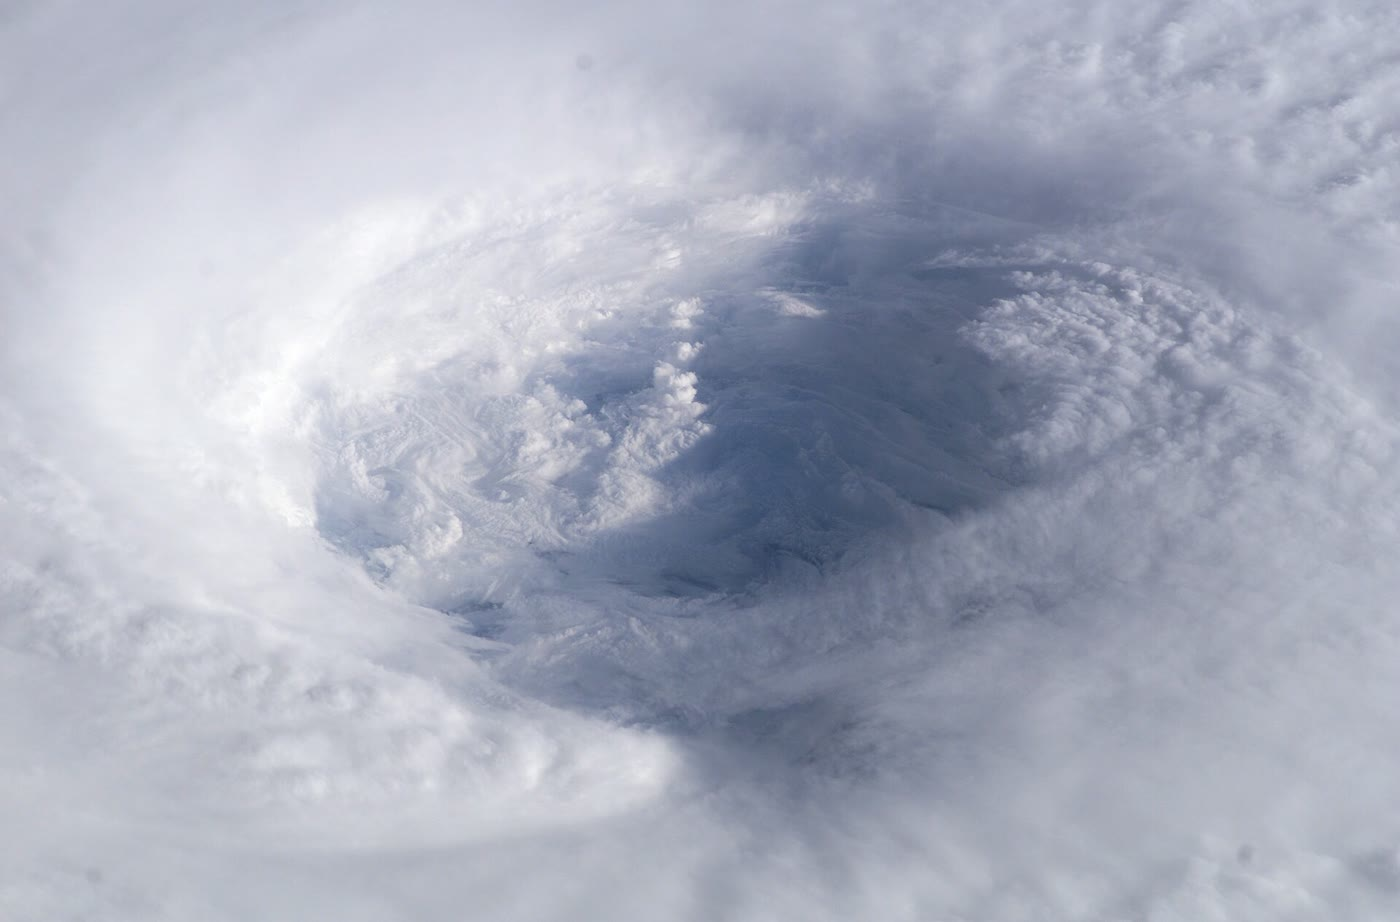
\includegraphics[width=0.62\linewidth]{images/book4/b2-22-isabel-eye.jpg}
\par\smallskip{\small Mata Badai Isabel, 13 September 2003, difoto dari
Stasiun Antariksa Internasional: dinding mata menurun seperti stadion ke awan rendah di dalam mata.
(Foto: astronaut NASA Ed Lu, domain publik, via Wikimedia Commons.)}
\end{omfigure}

\section{Prakiraan cuaca numerik}\label{sec:b2:weather-systems:nwp}

\begin{definition}[Prakiraan cuaca numerik; asimilasi data; prakiraan ensembel; batas keterprakiraan]\label{def:b2:weather-systems:nwp}
Yang disebut \emph{prakiraan cuaca numerik}\index{prakiraan cuaca numerik} adalah prakiraan dengan
komputer: persamaan-persamaan yang mengatur gerak, energi, dan air atmosfer
diintegralkan maju dalam waktu dari keadaan yang teramati. Yang disebut \emph{asimilasi data}\index{asimilasi data}
menggabungkan pengamatan terbaru dengan prakiraan jangka pendek dari pengamatan
sebelumnya untuk memperoleh perkiraan terbaik keadaan kini, yaitu analisis, yang menjadi titik awal
prakiraan. Yang disebut \emph{prakiraan ensembel}\index{prakiraan ensembel} adalah sekumpulan prakiraan yang dijalankan
dari keadaan awal yang sedikit berbeda, dan dengan versi model yang sedikit berbeda, untuk
menunjukkan rentang cuaca yang mungkin dan kemungkinannya. Yang disebut \emph{batas keterprakiraan}\index{batas keterprakiraan}
adalah waktu yang setelahnya prakiraan keadaan
cuaca tidak lebih baik daripada tebakan dari iklim, karena kesalahan keadaan awal telah
tumbuh sebesar selisih antara dua keadaan atmosfer mana pun.
\end{definition}
% ledger: nws4:nwp, ecmwf4:da, ecmwf4:ens-fs, krish19:predictability

Prakiraan numerik pertama dihitung pada 1950 dengan ENIAC, salah satu komputer elektronik
pertama. Model global masa kini membagi atmosfer menjadi kisi sel-sel yang berukuran beberapa kilometer
dan berangkat dari analisis yang memadukan pengamatan dari stasiun cuaca, pesawat terbang,
radiosonde, kapal, pelampung, dan, terutama, satelit, yang memberikan sumbangan terbesar bagi
kecakapan prakiraan global. Di sebuah pusat prakiraan besar, ensembelnya
memiliki 51 anggota, yaitu satu simulasi kontrol dan 50 simulasi yang diganggu, dengan resolusi sekitar \qty{9}{km}, yang dijalankan
dua kali sehari sampai 15 hari ke depan.
% ledger: krish19:predictability, ecmwf4:da, ecmwf4:ens

Mengapa mengganggu prakiraan yang dapat dimulai dari analisis terbaik? Karena atmosfer bersifat
kaotik, peka terhadap keadaan awalnya. Sebuah sistem tiga variabel, yang diterbitkan pada 1963, menunjukkannya
pada skala terkecil.

\begin{proposition}[Sistem Lorenz]\label{prop:b2:weather-systems:lorenz}
Sistem
\[
  \dot x = \sigma(y - x), \qquad \dot y = x(r - z) - y, \qquad \dot z = xy - bz,
\]
dengan $\sigma = 10$, $r = 28$, dan $b = 8/3$, memiliki sifat-sifat berikut.
\begin{enumerate}
  \item Titik-titik tetapnya adalah titik asal dan $C_\pm = \bigl(\pm\sqrt{b(r - 1)}, \pm\sqrt{b(r - 1)},
        r - 1\bigr) = (\pm 8.49, \pm 8.49, 27)$.
  \item Setiap volume dalam ruang fasenya menyusut sebagai $\mathrm{e}^{-(\sigma + 1 + b)t}$:
        lintasan-lintasannya berakhir pada himpunan bervolume nol, yaitu atraktor.
  \item Pada atraktor, dua lintasan yang berawal pada jarak kecil $\delta_0$ saling menjauh,
        rata-rata, sebagai $\delta(t) \approx \delta_0\,\mathrm{e}^{\lambda t}$, dengan $\lambda =
        0.906$, sampai $\delta$ mencapai ukuran atraktor (dihitung, diterima). Kesalahan
        kecil berlipat dua setiap $\ln 2/\lambda = 0.77$ satuan waktu.
\end{enumerate}
\end{proposition}
% ledger: nolitia22:lorenz

\begin{proof}[Bukti 1 dan 2]
Pada titik tetap, $y = x$ dari persamaan pertama; persamaan ketiga memberikan $z = x^2/b$; persamaan kedua
menjadi $x(r - 1 - x^2/b) = 0$, sehingga $x = 0$ atau $x^2 = b(r - 1) = 72$. Divergensi
medan vektor itu adalah $\partial_x\dot x + \partial_y\dot y + \partial_z\dot z = -\sigma - 1 - b$, sebuah
konstanta, dan menurut teorema divergensi, volume $V$ yang terbawa oleh aliran memenuhi $\dot V =
-(\sigma + 1 + b)V$.
\end{proof}

Gambar-gambar menunjukkan makna proposisi itu. Dua simulasi yang berawal dengan selisih \num{e-5} saling mengikuti
selama sekitar lima belas satuan waktu, lalu berpisah untuk selamanya: masing-masing masih tampak seperti
lintasan sistem yang masuk akal, tetapi keduanya bukan lagi lintasan yang sama. Dirata-ratakan atas 200 pasang
simulasi yang berawal dengan selisih \num{e-8}, jarak itu tumbuh secara eksponensial dengan laju $\lambda$, yaitu garis
lurus pada skala logaritmik, sampai jenuh pada ukuran atraktor. Berapa pun
kesalahan awalnya, kesalahan itu mencapai ukuran tersebut: kesalahan awal yang lebih kecil hanya menunda saat itu, sebesar
$\ln 10/\lambda = 2.5$ satuan waktu untuk setiap pengurangan sepuluh kali lipat.
% ledger: nolitia22:lorenz

\begin{omfigure}
\centering
% figdata/bachelor-2/weather.py parts traj, butterfly
\begin{tikzpicture}
\begin{groupplot}[group style={group size=2 by 1, horizontal sep=1.5cm},
  tick label style={font=\scriptsize}, label style={font=\small}]
\nextgroupplot[width=0.58\linewidth, height=5.0cm, xmin=0, xmax=30, ymin=-22, ymax=22,
  xlabel={waktu}, ylabel={$x$}, legend style={font=\scriptsize, at={(0.5,1.02)},
  anchor=south, draw=none, legend columns=2, /tikz/every even column/.append style={column
  sep=0.4cm}}, legend cell align=left]
\addplot[ocBlue, thin] table[x=t, y=x1] {figdata/out/bachelor-2-weather-traj.dat};
\addlegendentry{simulasi 1}
\addplot[ocRed, thin, densely dashed] table[x=t, y=x2] {figdata/out/bachelor-2-weather-traj.dat};
\addlegendentry{simulasi 2, berawal \num{e-5} darinya}
\nextgroupplot[width=0.4\linewidth, height=5.0cm, xmin=-22, xmax=22, ymin=0, ymax=52,
  xlabel={$x$}, ylabel={$z$}]
\addplot[black!70, very thin] table[x=x, y=z] {figdata/out/bachelor-2-weather-butterfly.dat};
\addplot[only marks, mark=*, mark size=1.3pt, ocRed] coordinates {(8.485,27) (-8.485,27)};
\end{groupplot}
\end{tikzpicture}
\par\smallskip{\small Sistem Lorenz ($\sigma = 10$, $r = 28$, $b = 8/3$), yang diintegralkan dengan
metode Runge--Kutta dengan langkah waktu 0.01. Kiri: dua simulasi yang berawal dengan selisih \num{e-5} dalam $x$
pada atraktor. Kanan: satu simulasi selama 40 satuan waktu, dilihat sepanjang $y$, dengan titik-titik tetap
$C_\pm$ (merah).}
\end{omfigure}
% ledger: nolitia22:lorenz

\begin{omfigure}
\centering
% figdata/bachelor-2/weather.py part growth
\begin{tikzpicture}
\begin{axis}[width=0.72\linewidth, height=5.6cm, xmin=0, xmax=30, ymode=log, ymin=1e-9,
  ymax=1e3, ytick={1e-9,1e-7,1e-5,1e-3,1e-1,1e1,1e3}, xlabel={waktu}, ylabel={jarak antara kedua simulasi}, tick label style={font=\scriptsize},
  label style={font=\small}, legend style={font=\scriptsize, at={(0.02,0.98)}, anchor=north west,
  draw=none, fill=none}, legend cell align=left, unbounded coords=discard, grid=major,
  grid style={black!8}]
\addplot[ocBlue, line width=1.6pt, opacity=0.55] table[x=t, y expr=10^\thisrow{log10d}]
  {figdata/out/bachelor-2-weather-growth.dat};
\addlegendentry{rata-rata 200 pasang (geometrik)}
\addplot[black, densely dashed, thin] table[x=t, y expr=10^\thisrow{fit}]
  {figdata/out/bachelor-2-weather-growth.dat};
\addlegendentry{eksponensial yang dicocokkan, $t = 2$ sampai 16}
\end{axis}
\end{tikzpicture}
\par\smallskip{\small Pertumbuhan jarak antara pasangan-pasangan simulasi sistem Lorenz yang berawal dengan selisih
\num{e-8}. Garis yang dicocokkan naik dengan faktor sepuluh setiap 2.57 satuan waktu, yaitu laju 0.897;
eksponen Lyapunov terbesar, yang dihitung dengan merenormalisasi satu pasang selama 2000 satuan waktu, adalah
0.909, dibandingkan dengan 0.906 yang diterbitkan. Pertumbuhan berhenti pada ukuran atraktor.}
\end{omfigure}
% ledger: nolitia22:lorenz

Atmosfer berperilaku dengan cara yang sama, dengan jauh lebih banyak variabel dan dengan kesalahan yang tumbuh dengan
laju berbeda pada skala yang berbeda. Dari prakiraan tahun 1980-an, kesalahan kecil ternyata
berlipat dua dalam sekitar 2.4 hari, dan prakiraan keadaan cuaca yang dapat diandalkan berhenti sebelum
sekitar sepuluh hari. Eksperimen yang memperkecil ketidakpastian keadaan awal masa kini, dengan model yang
dianggap sempurna, mendapati bahwa kondisi awal yang sempurna hanya akan menambah empat sampai lima hari, dan
bahwa pengurangan 90 persen sudah memberikan hampir semuanya: makin kecil kesalahannya, makin
cepat kesalahan itu tumbuh, melalui pelepasan kalor laten dalam konveksi, pada skala yang lebih kecil daripada yang dapat
diurai oleh prakiraan. \omterm{def:b2:weather-systems:nwp}{Batas keterprakiraan} di lintang tengah terletak sekitar dua minggu. Prakiraan
bertambah sekitar satu hari per dasawarsa karena pengamatan, asimilasi, dan model yang lebih baik membawanya
makin dekat ke batas itu; prakiraan tidak dapat melampauinya.
% ledger: krish19:predictability, selz22:limit, bauer:day-per-decade

Ensembel mengubah hal ini menjadi alat. Anggota-anggotanya berangkat dari analisis-analisis yang berbeda kira-kira
sebesar ketidakpastian analisis itu sendiri; selama anggota-anggota itu sepakat, prakiraannya tajam; ketika mereka
menyebar, prakiraan harus menyatakannya, dan prakiraan itu memberikan peluang. Prakiraan disebut andal bila
peristiwa yang diumumkannya dengan peluang \qty{70}{\percent} terjadi pada \qty{70}{\percent}
kasus.
% ledger: ecmwf4:ens-fs

\begin{inthelab}[Sehari di pusat prakiraan]
\begin{minipage}[t]{0.54\linewidth}\vspace{0pt}
Di pusat prakiraan global, hari berputar di sekitar dua waktu, 00 dan 12 UTC. Pengamatan yang berlaku
di sekitar setiap waktu itu berdatangan dalam jumlah jutaan, dari satelit, radiosonde, pesawat terbang, kapal,
pelampung, dan stasiun cuaca; \omterm{def:b2:weather-systems:nwp}{asimilasi data} memadukannya dengan prakiraan pendek sebelumnya menjadi
analisis. Model-model berangkat darinya, ensembel juga, dan prakiraan sampai ke penggunanya
beberapa jam kemudian, setelah superkomputer menjalankan 15 hari ke depan. Para prakirawan lalu
membandingkan simulasi-simulasi, memeriksanya terhadap pengamatan terbaru dan citra satelit, mengikuti
siklon dan front, dan mengubah peluang-peluang ensembel menjadi peringatan dan
prakiraan.
\end{minipage}\hfill
\begin{minipage}[t]{0.42\linewidth}\vspace{0pt}
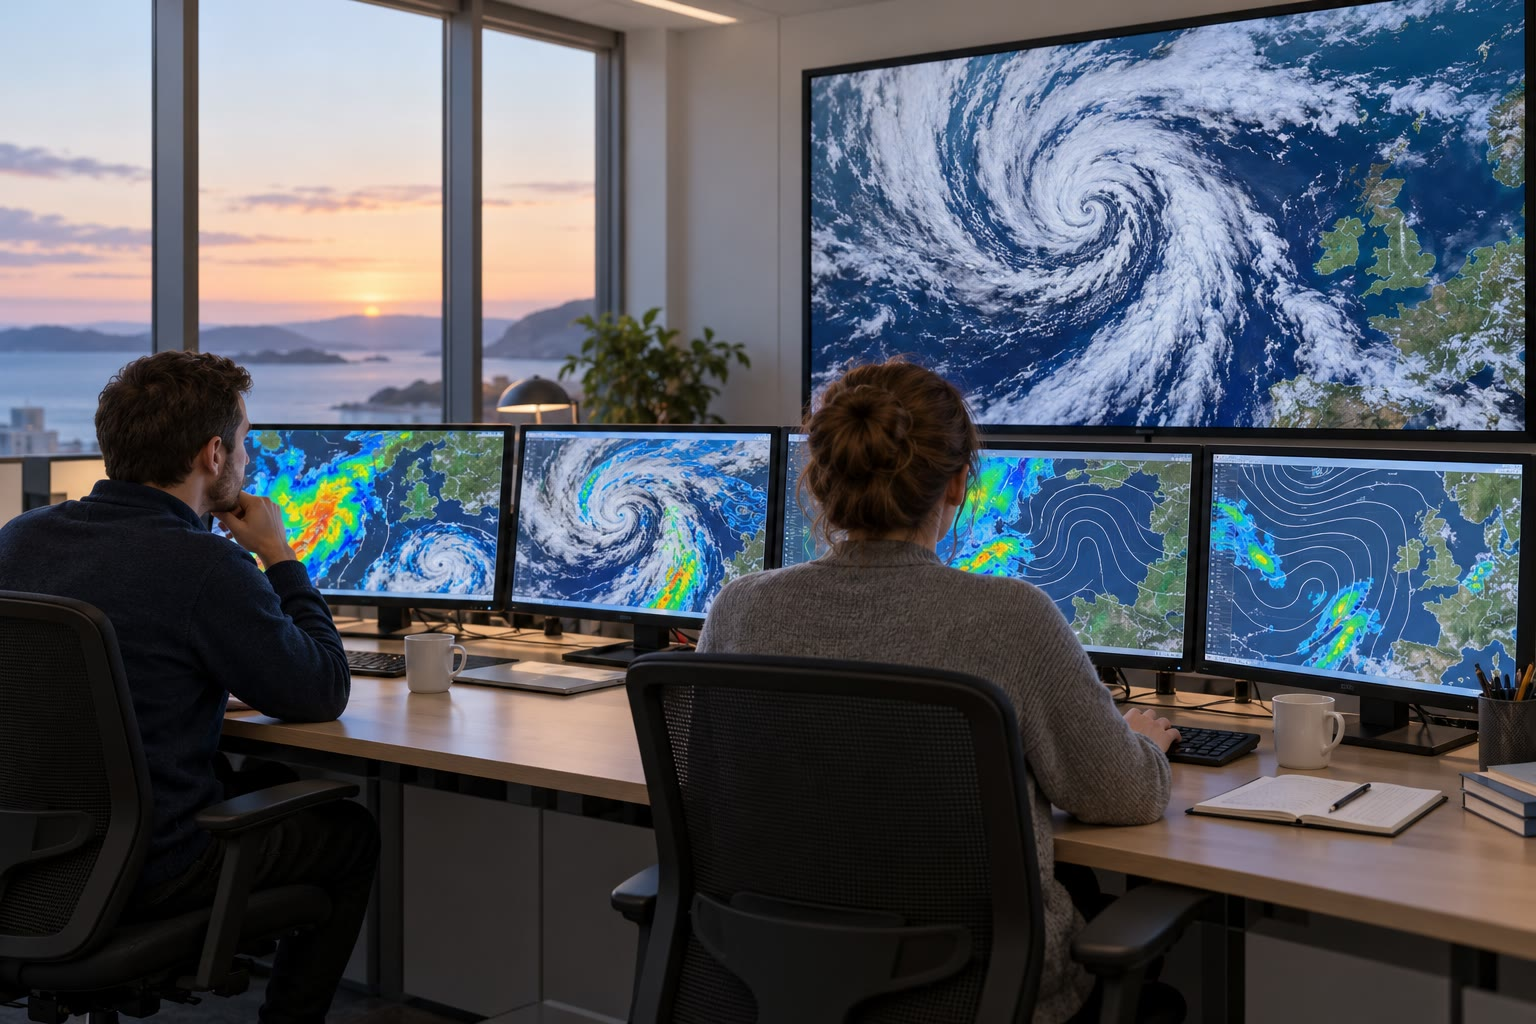
\includegraphics[width=\linewidth]{images/book4/ai/b2-forecast-office.jpg}

{\scriptsize Para prakirawan bekerja di depan citra satelit dan peta model
(ilustrasi buatan AI).}
\end{minipage}
% ledger: ecmwf4:ens, ecmwf4:da, mo:how-forecasts
\end{inthelab}

\section*{Latihan}\label{sec:b2:weather-systems:exercises}

Data untuk latihan, kecuali dinyatakan lain: $\Omega = \qty{7.292e-5}{s^{-1}}$, $a =
\qty{6371}{km}$, $g = \qty{9.81}{m.s^{-2}}$, $c_p = \qty{1004.5}{J.kg^{-1}.K^{-1}}$, $L =
\qty{2.501e6}{J/kg}$, dan \omterm{def:b2:atmospheric-thermodynamics:moist-air}{tekanan uap} jenuh pada latihan-latihan
\cref{ch:b2:atmospheric-thermodynamics}.
% ledger: earth:Trot, earth:Rmean

\begin{exercise}[$\star$]\label{exo:b2:weather-systems:1}
Pada \ang{50} LU sebuah front dingin memisahkan udara bersuhu \qty{275}{K} dari udara bersuhu \qty{281}{K}, dan angin
di sepanjangnya berubah \qty{15}{m/s}. (a) Hitunglah $f$. (b) Hitunglah kemiringan \omterm{def:b2:weather-systems:fronts}{bidang front},
sebagai 1 banding $N$. (c) Seberapa jauh di belakang front di permukaan tanah \omterm{def:b2:weather-systems:fronts}{bidang front} mencapai
\qty{1}{km}? (d) Apa yang terjadi pada kemiringannya jika kontras suhu berlipat dua dengan perubahan angin
yang sama?
\end{exercise}

\begin{exercise}[$\star$]\label{exo:b2:weather-systems:2}
\omterm{def:b2:weather-systems:fronts}{Bidang front} hangat naik dengan kemiringan 1 banding 150 dan bergerak dengan kecepatan \qty{25}{km/h}. (a) Seberapa jauh di depan
front di permukaan tanah \omterm{def:b2:weather-systems:fronts}{bidang front} berada \qty{6}{km} di atas? (b) Seorang pengamat melihat awan tinggi terbentuk
padanya di sana. Berapa lama kemudian front mencapai pengamat itu? (c) Gambarkan urutan
awan yang dilihat pengamat itu sementara itu.
\end{exercise}
% ledger: ucar:warm-front

\begin{exercise}[$\star$]\label{exo:b2:weather-systems:3}
Pada peta Belahan Bumi Utara, (a) sebuah garis dengan segitiga biru pada sisi tenggaranya membentang ke barat daya
dari suatu pusat tekanan rendah; (b) sebuah garis dengan setengah lingkaran merah pada sisi utaranya membentang ke timur dari pusat tekanan rendah yang sama; (c)
sebuah garis ungu dengan kedua simbol membentang dari pusat tekanan rendah lain ke titik tempat dua front lain bermula;
(d) sebuah garis berselang-seling antara segitiga biru pada sisi selatannya dan setengah lingkaran merah pada sisi utaranya.
Namailah setiap front, katakan di mana udara dingin berada dan ke arah mana masing-masing bergerak.
\end{exercise}
% ledger: ucar4:stationary-occluded, nws4:occluded

\begin{exercise}[$\star$]\label{exo:b2:weather-systems:4}
Pada \ang{45} LU dalam angin baratan \qty{12}{m/s}: (a) hitunglah $\beta$. (b) Hitunglah kecepatan fase
gelombang \qty{4000}{km} dan \qty{8000}{km}. (c) Ke arah mana masing-masing bergerak, dan seberapa jauh dalam
sehari?
\end{exercise}

\begin{exercise}[$\star\star$]\label{exo:b2:weather-systems:5}
(a) Tunjukkan bahwa \omterm{def:b2:weather-systems:rossby}{gelombang Rossby} diam dalam angin baratan $U$ bila $\lambda = 2\pi\sqrt{U/\beta}$.
(b) Hitunglah panjang gelombang itu pada \ang{45} LU untuk $U = \qty{12}{m/s}$. (c) Berapa banyak gelombang seperti itu yang muat mengelilingi
lingkaran lintang? (d) Mengapa angin baratan yang lebih kuat akan mendukung gelombang diam yang lebih sedikit dan lebih panjang?
\end{exercise}

\begin{exercise}[$\star\star$]\label{exo:b2:weather-systems:6}
Untuk sistem Lorenz: (a) periksalah bahwa $C_+$ adalah titik tetap dengan menghitung ketiga turunan
di sana. (b) Dengan faktor berapa sebuah volume kecil ruang fase menyusut dalam satu satuan waktu? (c) Mengapa
hal ini tidak mencegah dua lintasan yang berdekatan untuk saling menjauh?
\end{exercise}

\begin{exercise}[$\star\star$]\label{exo:b2:weather-systems:7}
Ambil $\lambda = 0.906$ untuk sistem Lorenz dan atraktor berukuran 10. (a) Hitunglah
waktu penggandaan kesalahan kecil. (b) Berapa lama kesalahan \num{e-8} mencapai ukuran
atraktor? (c) Seberapa lama kesalahan awal yang seribu kali lebih kecil menunda saat itu? Berapa
fraksi waktu yang ditemukan pada (b) itu?
\end{exercise}
% ledger: nolitia22:lorenz

\begin{exercise}[$\star\star$]\label{exo:b2:weather-systems:8}
Sebuah laut bersuhu \qty{303}{K} memiliki aliran keluar bersuhu \qty{195}{K}; ketidaksetimbangannya $h_o^* - h^* =
\qty{15}{kJ/kg}$ dan $C_k/C_D = 0.9$. (a) Hitunglah \omterm{prop:b2:weather-systems:pi}{intensitas potensialnya}. (b) Bandingkan dengan
ambang kategori 5 dan dengan badai tercepat belakangan ini. (c) Mengapa sebagian besar badai tidak mencapai
nilai itu?
\end{exercise}
% ledger: gilford21:pi, wk24:scale

\begin{exercise}[$\star\star$]\label{exo:b2:weather-systems:9}
Untuk badai pada \cref{exo:b2:weather-systems:8}: (a) hitunglah efisiensi Carnot mesin yang
bekerja antara permukaan laut dan aliran keluar. (b) Hitunglah faktor $(T_s - T_o)/T_o$ pada
\cref{prop:b2:weather-systems:pi} dan rasio keduanya. (c) Jelaskan perbedaannya.
\end{exercise}
% ledger: gilford21:pi

\begin{exercise}[$\star\star\star$]\label{exo:b2:weather-systems:10}
(a) Turunkan kembali \cref{prop:b2:weather-systems:slope} dengan mempertahankan densitas secara eksak, dan tunjukkan bahwa
udara dingin harus terletak di bawah. (b) Melintasi zona front selebar \qty{50}{km} pada \ang{45} LU, angin
di sepanjang front berubah \qty{10}{m/s}. Hitunglah vortisitas relatif zona itu dan bandingkan
dengan $f$. (c) Apakah zona itu siklonik atau antisiklonik?
\end{exercise}

\begin{exercise}[$\star\star\star$]\label{exo:b2:weather-systems:11}
Misalkan kesalahan prakiraan berlipat dua setiap 2.4 hari, berawal pada \qty{0.5}{K}, dan tidak berguna lagi pada
\qty{6}{K}. (a) Tentukan cakrawala prakiraan yang berguna. (b) Dengan faktor berapa kesalahan awal harus
mengecil setiap dasawarsa untuk memperoleh satu hari per dasawarsa, jika modelnya sempurna? (c) Eksperimen mendapati bahwa
kesalahan awal yang sepuluh kali lebih kecil hanya memberi tambahan 4 sampai 5 hari. Waktu penggandaan berapa yang tersirat untuk
kesalahan kecil, dan apa artinya tentang cara kesalahan kecil tumbuh?
\end{exercise}
% ledger: krish19:predictability, selz22:limit, bauer:day-per-decade

\begin{exercise}[$\star\star\star$]\label{exo:b2:weather-systems:12}
Ambil \cref{ex:b2:weather-systems:pi} dan hangatkan laut dan udara masing-masing \qty{1}{K}, dengan
kelembapan relatif dan suhu aliran keluar tidak berubah. (a) Hitung ulang $q_s^*$, $q_a$, dan
ketidaksetimbangannya. (b) Hitung ulang \omterm{prop:b2:weather-systems:pi}{intensitas potensialnya}. (c) Berapa persen per kelvin
intensitas itu naik, dan faktor mana yang paling banyak menyumbang?
\end{exercise}
% ledger: gilford21:pi

\begin{problem}[{Soal akhir pekan --- Seberapa jauh ke depan?}]\label{pb:b2:weather-systems:1}
Sebuah peta cuaca rekaan pada \ang{50} LU menunjukkan front dingin yang maju mendekati sebuah kota, dengan \omterm{def:b2:weather-systems:rossby}{gelombang Rossby}
dalam arus jet di atasnya. Soal ini mengikuti front itu, lalu gelombang itu, lalu menanyakan seberapa jauh
ke depan semuanya dapat diprakirakan. Gunakan data latihan.

\medskip\noindent\textbf{Bagian I --- Front.}
Pada pukul 06 UTC front dingin berada \qty{480}{km} di sebelah barat kota, pada pukul 12 UTC \qty{390}{km}. Di belakangnya
udara bersuhu \qty{277}{K}, di sektor hangat \qty{285}{K}, dan angin di sepanjang front
berubah \qty{16}{m/s} melintasinya.
\begin{enumerate}
  \item Tentukan kecepatan front itu.
  \item Pukul berapa front itu mencapai kota?
  \item Hitunglah $f$ pada \ang{50} LU.
  \item Hitunglah kemiringan \omterm{def:b2:weather-systems:fronts}{bidang front}.
  \item Seberapa tinggi \omterm{def:b2:weather-systems:fronts}{bidang front} di atas kota enam jam setelah front lewat?
  \item Berapa lama setelah front lewat udara dingin mencapai \qty{1.5}{km} di atas kota?
  \item Cuaca apa yang dialami kota ketika front lewat, dan bagaimana tekanan berubah?
\end{enumerate}

\medskip\noindent\textbf{Bagian II --- Gelombang di atas.}
Dalam arus jet di atas, angin baratan bertiup \qty{20}{m/s} dan gelombangnya memiliki panjang gelombang \qty{5000}{km}.
\begin{enumerate}[resume]
  \item Hitunglah $\beta$ pada \ang{50} LU.
  \item Hitunglah $k$ dan $\beta/k^2$.
  \item Tentukan kecepatan fase gelombang itu.
  \item Seberapa jauh sebuah palung bergerak dalam 24 jam?
  \item Tentukan panjang gelombang yang akan diam dalam angin ini, dan berapa banyak gelombang seperti itu yang muat
        mengelilingi \ang{50} LU.
  \item Di mana, relatif terhadap \omterm{def:b2:weather-systems:rossby}{palung udara atas}, siklon permukaan seharusnya mendalam?
\end{enumerate}

\medskip\noindent\textbf{Bagian III --- Atmosfer mainan.}
Pada gambar pertumbuhan kesalahan dalam sistem Lorenz, garis yang dicocokkan melalui
sekitar \num{5e-7} pada $t = 4$ dan \num{3.9e-3} pada $t = 14$.
\begin{enumerate}[resume]
  \item Dari kedua pembacaan ini, hitunglah laju pertumbuhan $\lambda$.
  \item Hitunglah waktu penggandaannya.
  \item Bandingkan dengan eksponen 0.906 yang diterbitkan.
  \item Mengapa jarak itu berhenti tumbuh, pada sekitar 15?
  \item Berapa lama lebih lambat kesalahan yang sepuluh kali lebih kecil mencapai ukuran itu?
\end{enumerate}

\medskip\noindent\textbf{Bagian IV --- Seberapa jauh ke depan?}
Ambil waktu penggandaan 2.4 hari yang ditemukan untuk kesalahan kecil pada prakiraan tahun 1980-an,
kesalahan awal \qty{0.1}{\celsius} pada suhu di suatu aras, dan prakiraan yang
tidak berguna lagi begitu kesalahan mencapai \qty{3}{\celsius}.
\begin{enumerate}[resume]
  \item Berapa kali penggandaan memisahkan kesalahan awal dari kesalahan yang tidak berguna?
  \item Berapa hari waktu yang diperlukan?
  \item Berapa hari yang akan diperoleh dengan membagi dua kesalahan awal?
  \item Dengan perkiraan lama waktu penggandaan 5 hari, cakrawala berapa yang akan diperoleh?
  \item Eksperimen modern mendapati bahwa kesalahan awal yang sepuluh kali lebih kecil, dan bahkan keadaan awal yang
        sempurna, hanya memberi tambahan 4 sampai 5 hari. Mengapa hal itu menunjukkan bahwa perkiraan pada
        pertanyaan~20 terlalu optimistis?
  \item Sebagai ringkasan: seberapa jauh ke depan, dalam hari, prakiraan ini dapat berguna?
\end{enumerate}
\end{problem}
% ledger: krish19:predictability, selz22:limit, nolitia22:lorenz, ucar:cold-front
